Researchers, service providers and security analysts have long been interested
in network and user behavioral patterns of the traffic crossing the internet
backbone. They want to use this information for the purpose of billing and
mediation, bandwidth provisioning, detecting malicious attacks, network
performance evaluation and overall improvement. Traffic measurement techniques
that have been rapidly evolving in the last decade, have matured enough today
to provide such an insight.

Flow capture today, has emerged out to be one of the favored network
measurement techniques. In this technique, packets traversing a monitoring
point are not captured raw, instead they are aggregated together based on some
common characteristics. The common characteristics are learnt by inspecting
the packet headers as they cross the monitoring point. Flow-records resulting
from such an aggregation are then exported to a collector for further
analysis. This not only reduces the amount of traffic at the monitoring point,
but also provides fine-grained control over the network data which was not
previously possible using SNMP interface-level queries.

NetFlow and \ac{IPFIX} are the two popular standards of IP flow information
export. NetFlow \cite{rfc3954} is a proprietary network protocol designed by
Cisco Systems. It allow routers to generate and export flow records to a
designated collector. NetFlow v$9$ provides flexibility of user-tailored
export templates, \ac{MPLS} and IPv$6$ support and a larger set of flow keys.
\ac{IPFIX} \cite{rfc5101} on the other hand is an open standard by IETF deemed
to be the logical successor of NetFlow v$9$ on which it is based. The novelty
of the standard lies in its ability to describe record formats at runtime
using templates based on an extensible and well-defined information model. The
data transfer mechanism is also simplistic and extensible by being
unidirectional and transport protocol agnostic.

The wide applicability of this approach is easily seen from the pervasive use
of flow records for a vibrant set of network analysis applications. For
instance, the authors in \cite{mkim:2004} use the flow characteristics in the
traffic pattern to formalize a detection function that maps traffic patterns
to different DoS attacks, whereas in \cite{sdominik:2010}, the authors
use the flow-record data to exploit timing characteristics of webmail clients
to classify features that could identify webmail traffic from any other
traffic running over HTTPS.

It goes to show that understanding these intricate traffic patterns require
sophisticated flow analysis tools that can mine flow records for such a usage.
Unfortunately current tools fail to deliver owing to their poor language
design and simplistic filtering methods.  We recently proposed a flow query
language design \cite{vmarinov:thesis:2009} that aims to cater to such needs.
It can process flow records, aggregate them into groups, apply absolute (or
relative) filters and invoke Allen interval algebra rules \cite{fallen:1983}.

In this paper, we introduce \ac{NFQL}, an efficient C implementation of the
flow query language. It is the next iteration of the first prototype
implementation, Flowy \cite{kkanev:2010}, which was written in Python.
\ac{NFQL} however is not just a reimplementation in a new language, but
the inner workings have been reimagined to allow the execution engine to
scale to real-world sized traces. This has been possible by replacing the
performance hit stages of the pipeline with crispier algorithms that lower
down the execution times to factor making them comparable to contemporary
flow analysis tools.

The rest of the paper is organized as follows. In section \ref{sec:design} we
describe the flow query language by discussing each stage of the processing
pipeline. In section \ref{sec:implementation} we introduce the inner workings
of \ac{NFQL}. It begins by providing an overview of the \ac{NFQL} components
and the structure of the intermediate format used to exchange messages. The
workflow of the execution engine is described next and is supplemented by a
number of performance optimizations made to make the implementation scale. It
is followed by performance evaluation results by comparing them against
contemporary flow processing tools in section \ref{sec:evaluation} and
concludes with a discussion on its current limitation and future outlook in
section \ref{sec:conclusion}.

\begin{figure*}[!t]
\centering
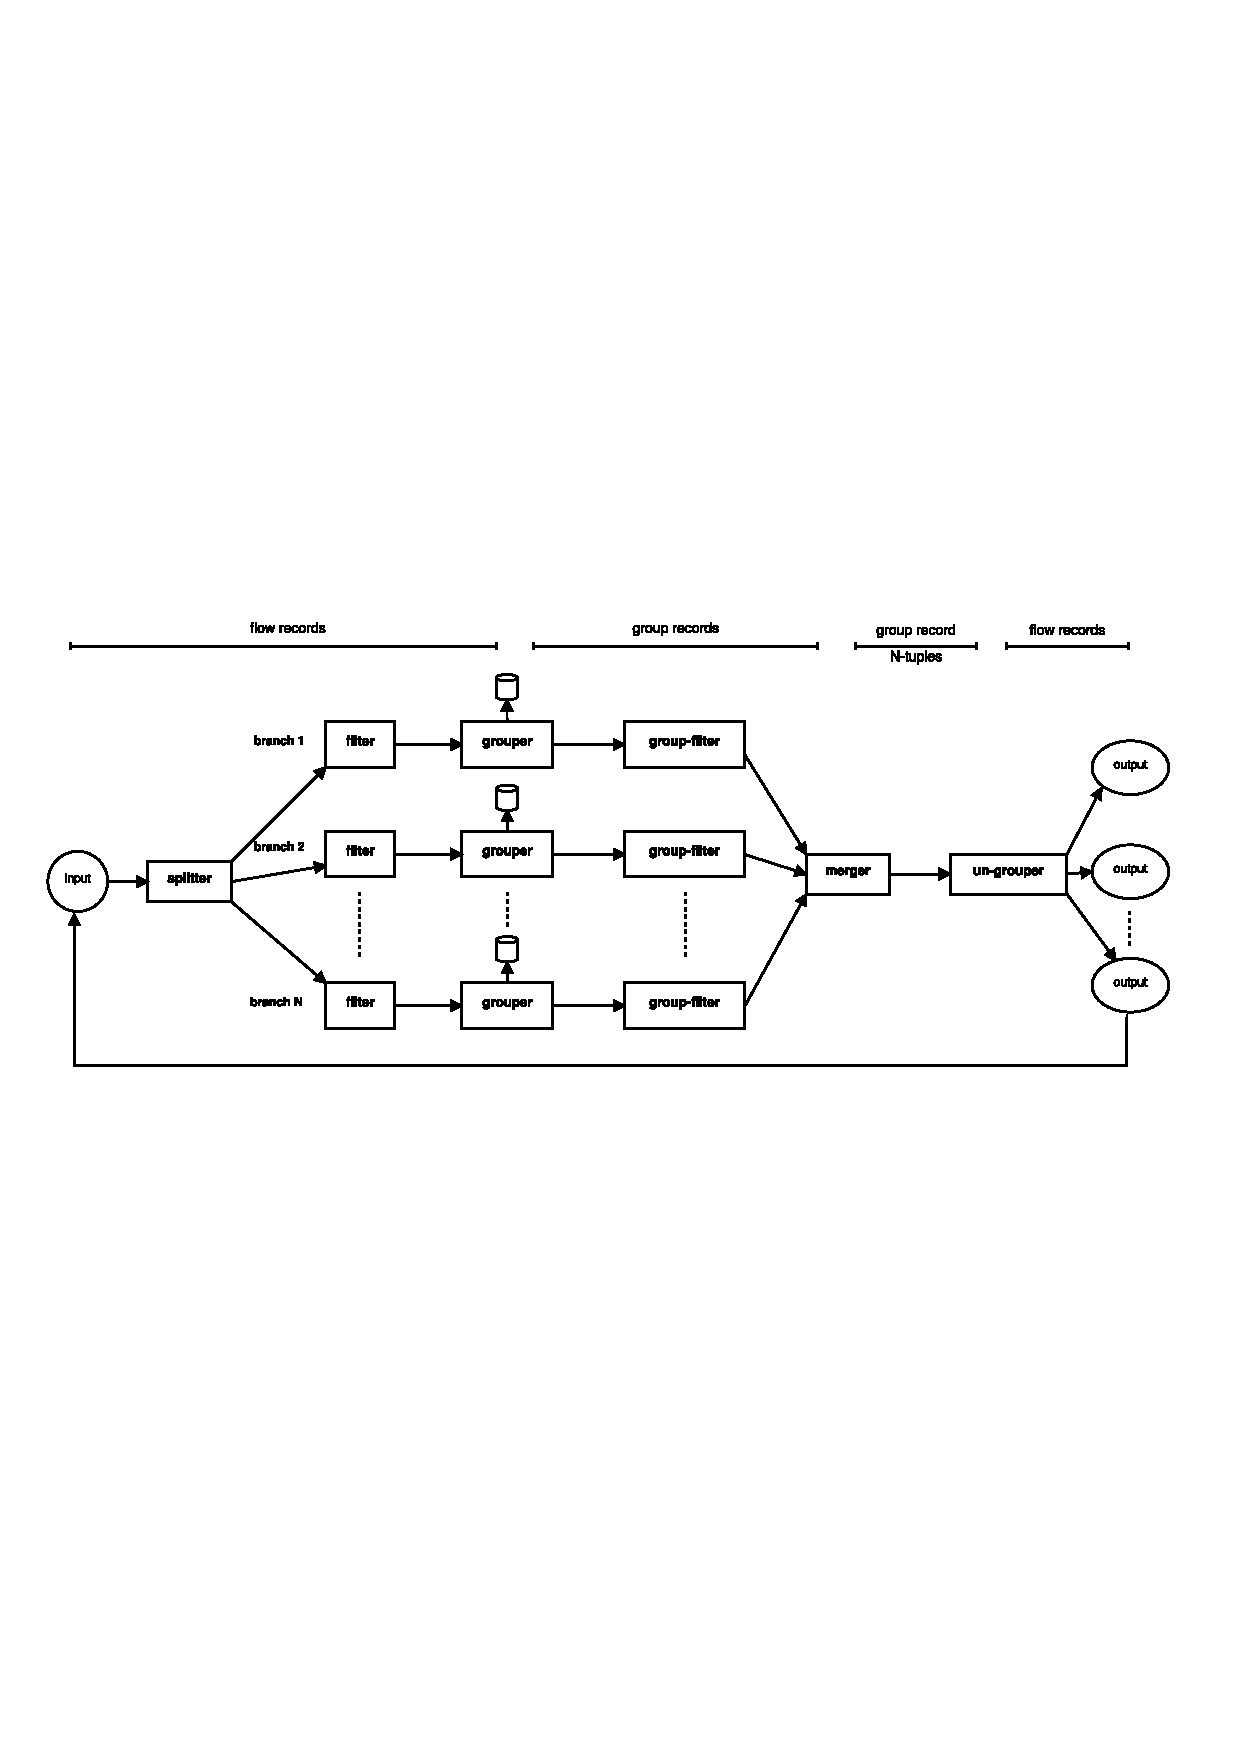
\includegraphics[width=0.9\linewidth]{nfql-pipeline}
\caption{NFQL Processing Pipeline \cite{vmarinov:2009}}
\label{fig:nfql-pipeline}
\end{figure*}
